%\documentclass[authoryear,round]{tufte-book}
\documentclass[a4paper,10pt]{article}
\usepackage[T1]{fontenc}
\usepackage[utf8]{inputenc}
\usepackage{amsmath}
\usepackage{amssymb}
\usepackage{graphicx}
\usepackage{fullpage}
\usepackage{color}
\usepackage{natbib}
\usepackage{mathrsfs}
\usepackage{array}
\newcommand{\head}[2]{\multicolumn{1}{>{\centering\arraybackslash}p{#1}}{#2}}
%\usepackage{sidecap}
\usepackage[capbesideposition={top,right},facing=yes,capbesidesep=quad]{floatrow}
\usepackage[hypertexnames=false]{hyperref}
\hypersetup{colorlinks=true, urlcolor=blue, citecolor=black, linkcolor=black}
%\usepackage{lineno}
%\usepackage{lscape}
%\usepackage{multirow}

\newcommand{\var}{\mathop{\mbox{Var}}}
\newcommand{\cov}{\mathop{\mbox{Cov}}}
\newcommand{\fancyN}{$\mathcal N$ }
\newcommand{\fancyB}{$\mathcal B$ }
\newcommand{\gc}[1]{{\it \color{red} (#1)} }
\newcommand{\jb}[1]{{\it\color{blue} (#1)} }
\def\citeapos#1{\citeauthor{#1}'s (\citeyear{#1})}
%\newcommand{\Rho}{\mathrm{P}}

%opening
\title{Theory of Sweeps from Standing Variation}
\author{
Jeremy J. Berg$^{1,2,3}$ and Graham Coop$^{1,2,3}$ \\
$^1$ Graduate Group in Population Biology, University of California, Davis. \\
$^2$ Center for Population Biology, University of California, Davis.\\
$^3$ Department of Evolution and Ecology, University of California, Davis\\
\small To whom correspondence should be addressed: \texttt{jjberg@ucdavis.edu, gmcoop@ucdavis.edu}\\
}

\date{}

\begin{document}

%\linenumbers
\maketitle

\begin{abstract}
\end{abstract}

%%%%%%%%%%%%%%%%%%%%%%%%%%%
\section{Introduction}



%%%%%%%%%%%%%%%%%%%%%%%%%%%
\section{Results}
Consider two loci, labeled \fancyN and \fancyB, which are separated on the chromosome by a recombination distance $r$. We imagine that an allele arises at the \fancyB locus and segregates at low frequency for some period of time (either due to neutral fluctuations, or because it is balanced at low frequency), before a change in the environment causes it to become beneficial and sweep to fixation. Alleles at the \fancyN locus are neutral, and its history can be determined by considering a structured neutral coalescent conditional on behavior of the \fancyB locus.

Our aim is to describe some features of the genealogy at the \fancyN locus, and to use this understanding of the genealogies to build intuition on the process of a sweep from standing variation, as well as to derive expectations for a range of population genetic summary statistics in a sample taken at the conclusion of a standing sweep.

The key insight for this paper is that the recombination events that occur between the \fancyN and \fancyB loci before the sweep has begun can be treated as mutations on the genealogy of the \fancyB locus, and thus under the assumption of constant population size, we can use the Ewens Sampling Formula to calculate expectations for a variety of quantities of interest in the region surrounding the selected site.

\jb{In this paper, we will use the phrase `beneficial allele' to refer to the allele that becomes beneficial during the selected phase and the phrase `non-beneficial allele' to refer to the complementary allele which becomes disfavored, regardless of whether the effect of selection is actually being felt during the part of the process being considered. We will use the phrase `sweep phase' to refer to the part of the history during which the beneficial allele is increasing in frequency due to positive selection, and the phrase `standing phase' to refer to the part of the history that preceeds the onset of selection.}

\begin{figure}
	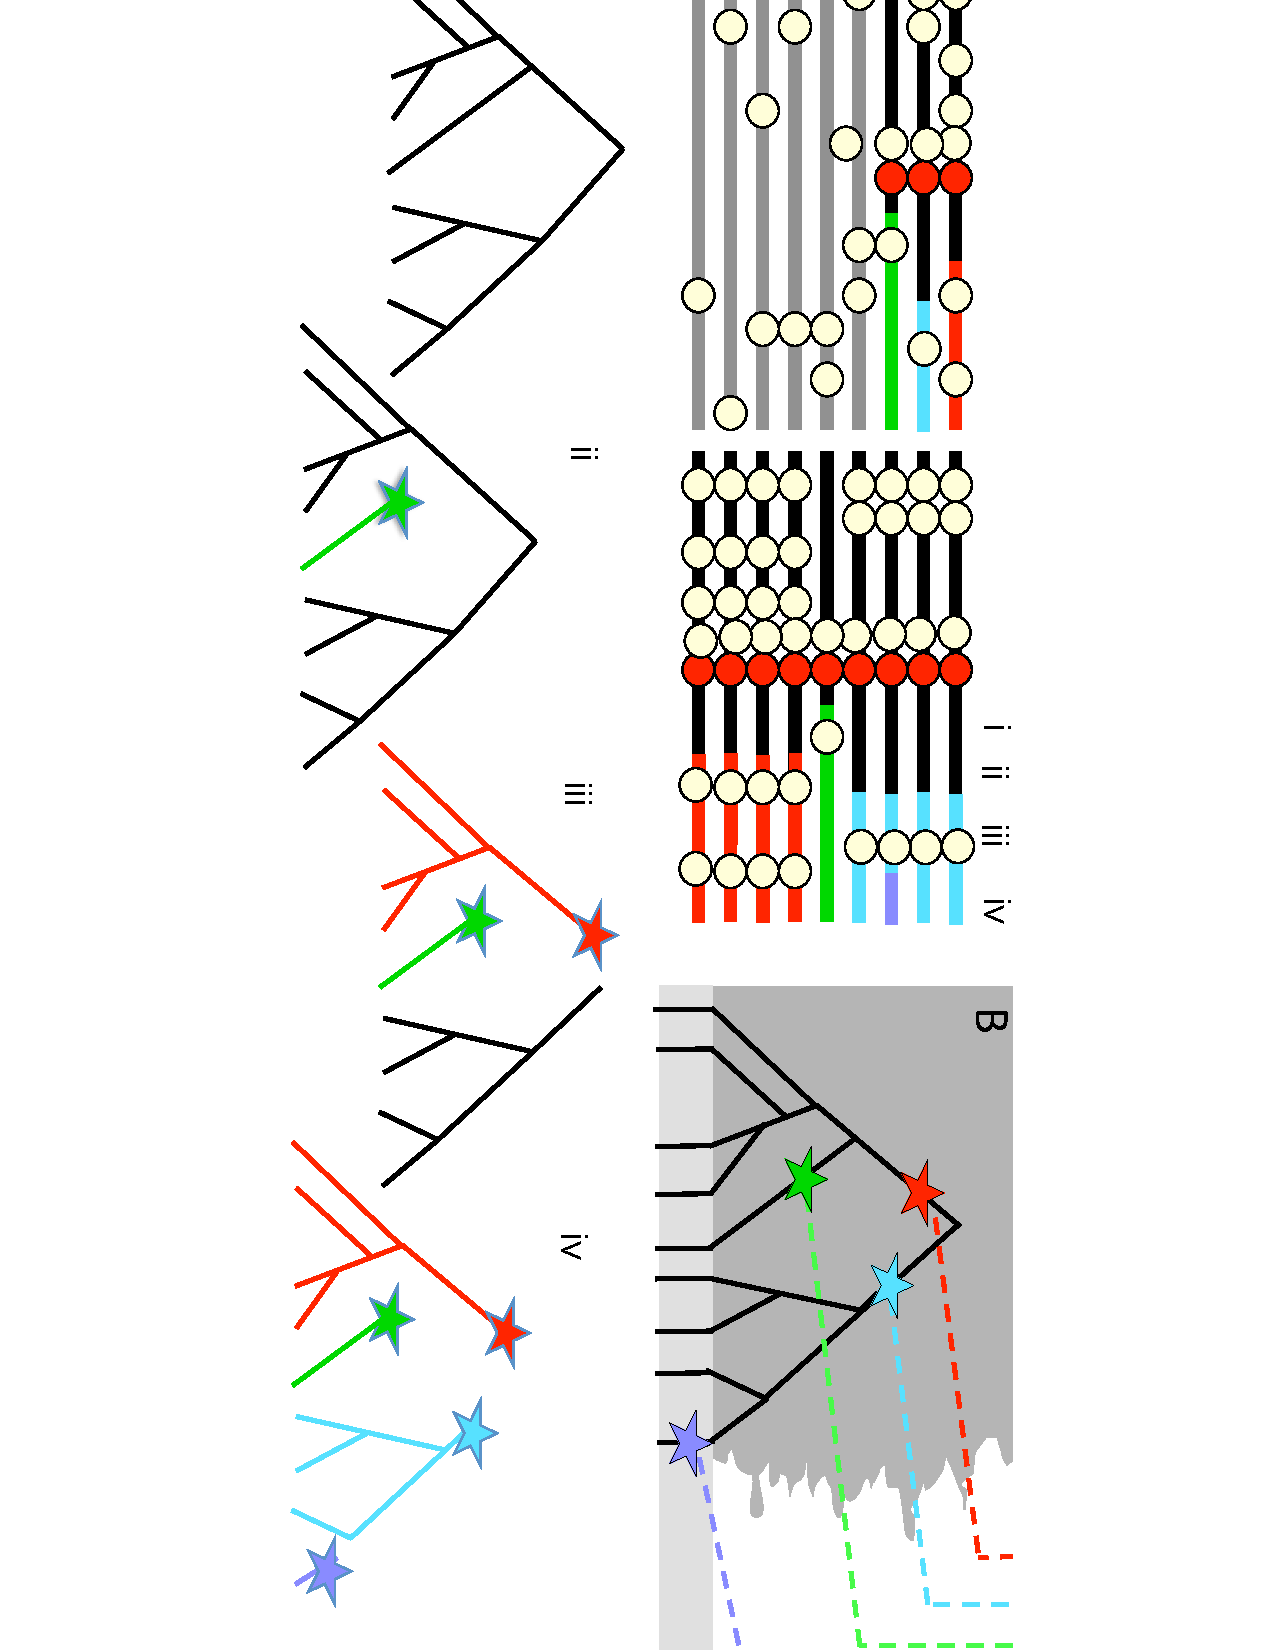
\includegraphics[width = 0.8\textwidth]{../Paper_Figures/Cartoon_of_soft_sweeps.pdf} \label{cartoon_fig_1}
	\caption{caption goes here}
\end{figure}


\subsubsection{Sweep Phase}
Looking backward in time, we let $X\left(t\right)$ be the frequency of the beneficial allele at the \fancyB locus at time $t$ in the past, where $t=0$ is the moment of fixation (i.e. $X\left(0\right) = 1; X\left(t\right) < 1\ \forall\ t > 0$). The probability that a single lineage sampled at the \fancyN locus at $t=0$ fails to recombine off of the selected background in generation $t$ is $1-r\left(1-X(t)\right)$. If we let $\tau$ be the first generation (forward in time) in which the allele at the \fancyB locus is beneficial (i.e. $X\left(\tau\right) = f$), then the probability that a single lineage manages to recombine off the selected background at any point during the course of the sweep is given by
\begin{equation}
P_{NR} = \prod_{t=0}^{\tau} 1-r\left(1-X(t)\right)  \approx \exp \left(-r \int_0^{\tau}(1-X\left(t\right))\mathrm{d} t \right)
\end{equation}
for $r \ll 1$. We set  $\mathcal{T}_{\left(s,f\right)} = \int_0^{\tau}(1-X\left(t\right))\mathrm{d}t$, so that the probability that a lineage manages to recombine off the selected background during the course of the sweep from frequency $f$ can be written $e^{-r\mathcal{T}_{\left(s,f\right)}}$. If the effect of our beneficial allele on relative fitness is strictly additive, such that heterozygotes enjoy a selective advantage of $s/2$ and heterozygotes an advantage of $s$, then the trajectory of the beneficial allele through the population can be approximated deterministically by the logistic, such that 
\begin{equation}
	\mathcal{T}_{\left(s,f\right)} = \frac{ln\left(\frac{N_e - 1}{f}-N_e + 1\right)}{s} \textrm{\jb{this is the 1/2N approx}}
\end{equation}

We assume that the sweep occurs fast enough that the probability of coalescence during the sweep is essentially zero. Therefore, each lineage makes an independent choice of whether it recombines out of the sweep, so that the probability that $i$ out of $n$ lineages fail to escape off the sweep background is
\begin{equation}
P_{NR}(i;n) = {n \choose i} P_{NR}^{i} (1-P_{NR})^{n-i}.
\end{equation}
This binomial approximation has been made by a number of authors in the context of hard sweeps \citep{Barton}, and more accurate approximations have been developed \citep{Etheridge2006}. However, as long as the population is large, the sample is not too large,  and $\tau$ is not too long, then this approximation should be adequate. Other, more accurate approximations could certainly be incorporated into our framework, but we stick with this simple form for the sake of clarity of presentation.

%At a given distance away from the selected site every one of the lineages that recombines out of the selected class will be a singleton, and the remaining lineages will be partitioned according to the Ewens' Sampling formula.  



\subsubsection{Standing Phase}
Looking backward in time, having originally sampled $n$ lineages at the \fancyN locus at $t=0$, we arrive at the beginning of the standing phase at time $\tau$ with $n-i$ lineages linked to the non-beneficial background at the \fancyB locus (which has a frequency of $1-f$), and $i$ lineages linked to the beneficial background (which has a frequency of $f$). We will argue that an understanding of patterns of neutral diversity at the \fancyN locus following the sweep can be obtained principally by considering the genealogy at the \fancyB locus, and then considering the effect of recombination events which occur in between the \fancyB and \fancyN loci conditional on this genealogy. The following paragraphs are therefore structured as follows: first, we describe an approximation to the coalescent process at the \fancyB locus conditional on being at a frequency $f$ at the beginning of the standing phase. Next, we describe an approximation to the process of recombination events which move alleles at the \fancyN locus from the beneficial background onto the non-beneficial background at the \fancyB locus. Finally, we combine these two processes along with the recombination process during the sweep phase and a separation of timescales argument to give an approximate description of the full genealogy at the \fancyN locus.

\paragraph{The Coalescent Process at the \fancyB Locus}

In attempting to construct the genealogy of the \fancyB locus backward in time, consider that in the first generation of the standing phase, the instantaneous pairwise coalescence rate of beneficial alleles is $1/\left(2Nf\right)$, such that the total rate of coalescence of beneficial alleles in the sample for the first generation is ${i \choose 2}/\left(2Nf\right)$. If the beneficial allele were held fixed at this frequency $f$ over a long period into the past, then the genealogy of our $i$ beneficial lineages would simply be a neutral coalescent with pairwise coalescent rate $1/(2 N f)$ (assuming that $f \gg 1/(2N)$ so that the standard coalescent assumptions hold). Such a fixed frequency could result from a beneficial allele that was balanced at low frequency by strong, constant selection. If instead of being held steady at a frequency $f$, the allele is allowed to drift neutrally, this constant coalescent rate no longer holds, and the problem becomes considerably more complicated.

A number of researchers have studied the behavior of this process \citep{XXXX}, either conditional on the frequency of the allele in a sample or in the population. \cite{Wiuf:2000js} has shown that the expected time to the first coalescent event is $2 N f/ {i \choose 2}$ in the absence of other information, e.g. as to whether the allele is ancestral or derived. However, the distribution of coalescence times is no longer exponential. The variance of the time between coalescent events is increased relative to the exponential as a direct result of the fact that the frequency may increase or decrease from $f$ before a given coalescent event is reached. Further, in contrast to the standard coalescent, there is non-zero covariance between subsequent coalescent intervals, as a result of the fact that early coalescent events contain information about how the frequency of the allele has changed, and thus about the rate at which subsequent coalescent events occur. Lastly, if the allele is known to be either derived or ancestral the coalescent times have a more complicated expectation, as the allele is in expectation either decreasing or increasing in frequency backward in time due to the conditioning on loss or fixation respectively.

Despite these complications we have found assuming that lineages coalesce at a rate $ {i \choose 2}/(2 N f)$ and that coalescent time intervals are independent, i.e. that the allele frequency does not drift from $f$, is not a bad approximation when $f \ll 1$ regardless of whether the allele is ancestral or derived. In Supp. Figures XXX-XXX we show some comparisons of the coalescent process embedded in a drifting allele frequency and this approximation. 

The main reason for using this approximation is that it allows us to work with a simple, well understood caricature of the true process that describes the genealogy at the selected site with reasonable accuracy. Conditional on this simplified coalescent process, we can study the process of recombination events occurring between the \fancyB and \fancyN loci to understand the distribution of the genetic variation at the \fancyN locus that will hitchhike along with the beneficial allele once the sweep begins. 

\paragraph{Recombination Between \fancyB and \fancyN}
We will again rely on the condition that $f \ll 1$, and assume that any lineage at the \fancyN locus that recombines off of the background of our beneficial allele will not recombine back into that background before it is removed by mutation. Under these assumptions, recombination events which move lineages at the \fancyN locus from the beneficial background onto the non-beneficial background can be viewed as events on the genealogy at the \fancyB locus which occur at rate $r\left(1-f\right)$ per lineage. Rescaling time by $2Nf$, an understanding of the genealogy at the \fancyN locus can therefore be found by considering the competing poisson processes of coalescence at rate ${i \choose 2}$, and recombination at total rate $2Nirf(1-f)$

%In Figure \ref{cartoon_fig_1}B we show the coalescent genealogy at the selected site, and show recombination events out of the beneficial allele class imposed on the genealogy (these events are colored to correspond to the events on the haplotypes in Figure \ref{cartoon_fig_1}A). In Figure \ref{cartoon_fig_1}C we show the genealogy at various points along the sequence shown in Figure \ref{cartoon_fig_1}A, between recombination events. 

%Assuming that the frequency of the allele remains fixed at $f$, at a distance $r$ away from the selected site a lineage recombines out of the selected class at rate $r(1-f)$. As coalescent occurs at a rate ${i \choose 2}/(2Nf)$, we can rescale time in units of $2Nf$ so that coalescence happens at a rate ${i \choose 2}$, and recombination events out of the selected class happen at rate $2Nrf(1-f)$.

If we are interested in the number and size of different recombinant clades at a given recombination distance from the selected site (colored clades in Figure \ref{cartoon_fig_1}B \& C)  this a direct analogy of the infinitely-many allele model \citep{}. In the infinite alleles model, every mutation event creates a new allele, while in our process every recombination event creates a new recombinant lineage (an potentially a distinct haplotype, depending on the configuration of mutations). Further, a sample from the infinite alleles process can be found by simulating the coalescent, scattering mutations down on the genealogy, and then assigning each lineage to be of a type corresponding to the mutation that sits lowest above it in the genealogy (see Figure \ref{cartoon_fig_1}B). Equivalently, we can create a sample under the infinite allele model by simulating the mutational and coalescent processes simultaneously, `killing' lineages whenever they first encounter a mutation and assigning all tips sitting below the mutation to be of the same allelic type (see Figure \ref{cartoon_fig_1}C). 

Given the direct analogy to the infinite alleles model under our set of approximations, the number and frequency of the various recombinant lineage classes at a given distance from the selected site can be found using the Ewens' Sampling Formula \citep[ESF][]{}.The population-scaled mutation rate in the infinitely-many alleles model ($\theta/2=2N\mu$), in our model, is replaced by the rate of recombination out of the selected class ($R_{f}/2=2Nrf(1-f)$). If $i$ lineages sampled at the moment of fixation fail to recombine off of the beneficial background during the course of the sweep, then the probability that these $i$ lineages coalesce into a set of $k$ recombinant lineages is 
\begin{equation}
	p_{ESF}(k \mid R_f,n)  = S(i,k) \frac{R_f^k}{ \prod_{\ell=1}^{i-1} (R_f +\ell) }  \label{ESF1}
\end{equation}
where $S(i,k)$ is a Stirling number of the first kind
\begin{equation}
	S(i,k) = \sum_{i_1 + \dots + i_k = i} \frac{i!}{k!i_1\dots i_k}
\end{equation}
These recombinant lineages partition our sample up between themselves, such that each lineage has some number descendants in our present sample$\{i_1,i_2,\dots,i_k\}$, where $\sum_{j=1}^k i_j =i$. Conditional on $k$ the probability of a given sample configuration is
\begin{equation}
	p(\{i_1,i_2,\dots,i_k\} \mid k,i) = \frac{i!}{k! i_1\cdots i_k S(i,k)}  \label{ESF2}
\end{equation}
Note this does not depend on $R_f$, which gives the classic result that the number of alleles is sufficient statistic for $R_f$ (i.e. the partition is not needed to estimate $R_f$).

\jb{Formally, we consider a limit in which $f$ tends to zero while $N$ tends to infinity such that $2Nf$ is held constant at some value much larger than one. This results in a separation of timescales where both coalescent and recombination events on the background of the beneficial allele occur nearly instantaneously relative to events on the background of the non-beneficial allele.}

\begin{figure}
	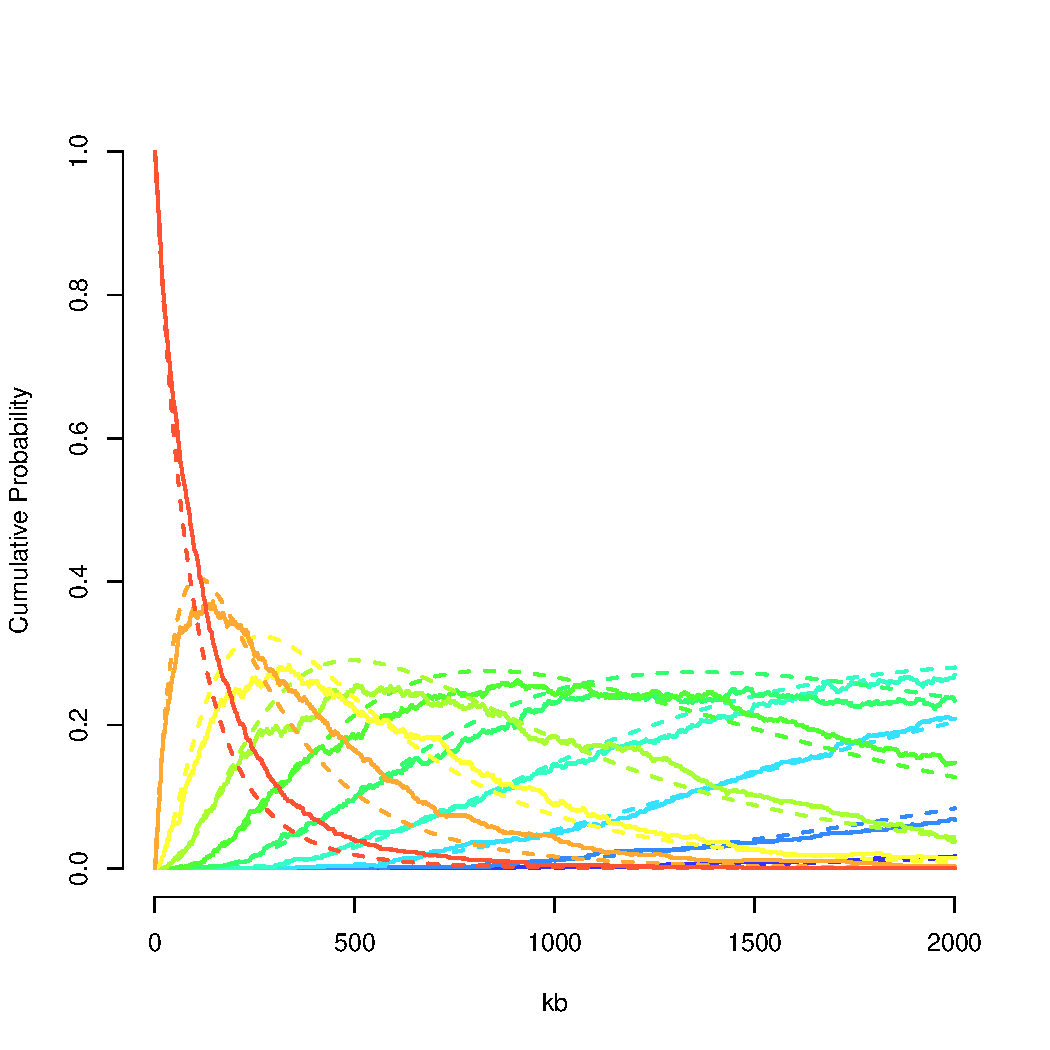
\includegraphics[width = 0.8\textwidth]{../Paper_Figures/Ewens_vs_Jeremy.pdf}
\end{figure}

%and that the number of coalescent families with $1,2,\dots,n$ lineages is given by the partition
%  $\{n_1,n_2,\dots,n_k\}$ is 
% \begin{equation}
% P\left(k,n_1,n_2,\dots,n_n\mid R_f,n \right) =\frac{R_f^i}{ \prod_{j=1}^{i-1} (R_f +j) } \prod_{j=1}^n\frac{1}{j^{n_j}n_j!} \label{ESF}
% \end{equation}
% The probability of there being $k$ alleles (recombinant lineages) in our sample of $n$

\subsubsection{Patterns of neutral diversity surrounding standing sweeps}
Given this approximate model of the coalescent with a sweep from standing variation we can now calculate basic summaries of variation in the region surrounding the sweep. We will assume that the per base pair mutation rate per generation is $\mu$. We will ignore mutations over the time-scale of our shrunken coalescent tree, and assume that all diversity comes from mutations that occurred prior to the sweep, or equivalently that this part of the genealogy contributes neglibably to the total amount of time in the genealogy. This corresponds to an assumption that $2N\mu \gg 2N \mu f$, in line with our previous set of assumptions that $f \ll 1$. If this is the case we simply consider patterns of diversity in our sample at a site, by considering properties of the recombinant lineages in our sample, which correspond to alleles drawn independently from a neutral population prior to the start of our sweep.

For example, excluding recombination during the sweep for a moment, the expected pairwise coalescent time a distance $r$ away from our sweep is
\begin{equation}
	\mathbb{E}(T_2)\approx \frac{1}{1 + 4Nrf(1-f)} \times 0 + \frac{4Nrf(1-f)}{1 + 4Nrf(1-f)} \times 2N
\end{equation}
where the two terms correspond to the contribution from failing to recombine during the standing phase and so coalescing very rapidly, and alternately to one or both lineages escaping from the beneficial background and coalescing $2N$ generations ago. In Figure XXX we show this approximation, and coalescent simulations done using $ms$. 

Now incorporating recombination during the sweep our expected pairwise coalescent time a distance $r$ away from our sweep is 
\begin{equation}
	\mathbb{E}(T_2) \approx \left(1-\frac{1}{1 + 4Nrf(1-f)} P_{NR}^2  \right) \times 2N
\end{equation}
as to avoid (near) instantaneous coalescence our pair of lineages could recombine during either the sweep or standing phases. The expected level of pairwise diversity as we move away from a sweep is given by $2\mu \mathbb{E}(T_2)$

We can extend this idea of conditioning on the number of lineages that escape the sweep to calculate the expected total time in the genealogy as we move away from the \fancyB locus. Conditional on  $k$ independent lineages escaping the sweep, the expected total time in the genealogy is $2N \sum_{\ell=1}^{k-1} 1/\ell$, the standard result for a neutral coalescent with $k$ lineages \citep{Watterson}. Ignoring for a moment recombination during the sweep phase, the probability that $k$ lineages escape the sweep is the probability of $k$ alleles in a sample of $n$ under the ESF $p_{ESF}(k\mid R_f,n)$ (under our approximation). The expected time in the genealogy a distance $r$ away from the selected site is therefore
\begin{equation}
	\mathbb{E}(T_{TOT})  \approx 2N \sum_{k=2}^n p_{ESF}(k\mid R_f,n)   \sum_{j=1}^{k-1} 1/j
\end{equation}
In Figure XXX we show this approximation, and coalescent simulations done using $ms$. 

%\begin{figure}
%\includegraphics[width = 0.8
%          \textwidth]{Paper_Figures/pi_density.pdf}
%\end{figure}
%
%\begin{figure}
%\includegraphics[width = 0.8
%          \textwidth]{Paper_Figures/segsite_density.pdf}
%\end{figure}

Reincorporating recombination during the sweep phase, the probability that $k$ distinct lineages have recombined off of the beneficial background between the two phases together is
\begin{equation}
	\sum_{m=0}^{k} {n \choose m} P_{NR}^{m} (1-P_{NR})^{n-m} p_{ESF}\left(k-m\mid R_f, n-m\right),
\end{equation}
as if we generate $m$ recombinant lineages during our sweep, then the remaining $k-m$ recombinant lineages have to come from recombination events in the standing phase (we set $p_{ESF}\left(0,R_f,0\right)=1$, representing the extreme case where $k=n$ and all lineages manage to recombine during the sweep phase). The expected total time in the genealogy is therefore
\begin{equation}
\mathbb{E}(T_{TOT})  \approx 2N\sum_{m=0}^{k} {n \choose m} P_{NR}^{m} (1-P_{NR})^{n-m} p_{ESF}\left(k-m\mid R_f, n-m\right)   \sum_{\ell=1}^{k-1} 1/\ell
\end{equation}
and the expected number of segregating sites can be found by taking $\mu$ times this. 

We can also obtain an expression for the frequency spectrum at sites surrounding a standing sweep. To break the problem into approachable components, we condition on an absence of recombination during the sweep phase, and a fixed number $k$ recombinant families which are created by coalescence and recombination in the standing phase (both of these will be relaxed momentarily). Each of the $k$ recombinant families represents an independent draw from the population frequency prior to the beneficial allele at the \fancyB locus entering the population. If we condition on $j$ out of $k$ recombinant lineages carrying a derived allele, then we can obtain the probability that $l$ of the $n$ lineages sampled at fixation carry the derived allele by summing over all possible partitions of the $n$ tips into $k$ families such that the $j$ recombinant ancestors carrying the derived mutation have exactly $l$ descendants in the present day as
\begin{equation}
p(l \mid j, ~k,~i=n) = \sum_{\substack{i_1+\cdots +i_j=l \\i_{j+1}+\cdots + i_k=n-l}} p(\{i_1,\dots,i_k\} \mid k, n) = \frac{ {n \choose l} }{ {k \choose l} }\frac{ S(l,j)  S(n-l,k-j)  }{ S(n,k) } \label{ESF_gives_freq_spec}
\end{equation}

Next, we write $q_{j,k}$ to denote the probability that $j$ out of the $k$ recombinant families carry the derived mutation. For our purposes, we will assume this distribution follows that of the standard neutral coalescent expectation (such that $q(j \mid k) = \frac{1/j}{\sum_{\ell=1}^{k-1}1/\ell}$ gives the probability of $j$ derived alleles in a sample of $k$, conditional on segregation), although one could easily use an empirical frequency spectrum measured from genome-wide data, as in \citep{NielsenKim}. The probability that the derived allele is present in $l$ out of $n$ sampled lineages, conditional on there having been $k$ recombinant families, is then $p(l \mid ~k, ~i = n ) = \sum_{j=1}^k p(l \mid j,~k, ~n)q(j\mid k)$. Summing over the distribution of $k$ given by \eqref{ESF1}, we obtain an expression for the frequency spectrum ignoring recombination in the sweep phase as
\begin{equation}
p(l \mid i=n) =  \sum_{k=1}^{n}  p_{ESF}(k \mid R_f,n)  \sum_{j=1}^k p(l \mid j,~k, ~n)q(j\mid k)
\end{equation}
%
%To do this we make use of a trick borrowed from \cite{Kimandstephan}, and subsequently used by \cite{NielsenKimetc}, where the frequency spectrum after a sweep reflects the fact that $k$ recombinant lineages survive through the sweep and these $k$ lineages reflect independent draws from the population frequency. This trick was also used by \cite{Pennings:2006fs} to obtain the frequency spectrum of fully linked variation surrounding a soft sweep from multiple mutations (see the ``Frequency distribution of ancestral variation'' subsection in their ``Analytical Derivations'' section). We will denote the probability of sampling $j$ derived copies of a neutral allele out of a sample of $k$ by $q_{j,k}$, i.e. the neutral frequency spectrum in a sample of $k$. At a neutral site at demographic equilibrium $q_{j,k} = 1/j$ \gc{actually what do we want to do here? Do we want site to be segregating? }, otherwise it could be replaced by the empirical frequency spectrum calculated genome-wide \citep[as in ][]{NielsenKimetc}
%Consider the case where no recombination occurs during the selected phase, in that case the probability of observing a neutral site segregating at a frequency of $l/n$ can be written as
%\begin{equation}
%p(l \mid n) =  \sum_{k=1}^{n}  p_{ESF}(k \mid R_f,n)  \sum_{j=1}^{k} q_{j,k}  p(l \mid k,n) 
%\end{equation}
%where $  p(l \mid k,n) $ is the probability that our $k$ recombinant lineages lead to a sample containing into $l$ derived alleles and $n-l$ alleles when the neutral allele segregates at a frequency of $j/k$ in the population before the sweep. To find this we have to sum over the possible configurations $\{a_1,\dots,a_k\}$ as follows

When we allow for recombination during the sweep this expression becomes more complex, but the same logic can be followed and write
\begin{equation}
p(l \mid n) = \sum_{i=0}^n P_{NR}(i\mid  n) \sum_{k=1}^{i} P_{ESF}(k \mid R_f,n-S) \sum_{j=1}^{k+n-i-1} q(j\mid k+n-i) \sum_{i=1}^{l \wedge \left(n-i\right)} H(g \mid j,k,n-i) p(l-g \mid j-g,k,n-i)
\end{equation}
where A$\wedge$B denotes min(A,B) and
\begin{equation}
	H(g \mid j,k,n-i) = \frac{{j \choose g}{n-i \choose g}}{{k + n - i \choose j}}
\end{equation}
gives the probability that $g$ out of $j$ derived alleles are found on singleton recombinants created during the sweep, given that there are $n-i$ singletons, and $k$ recombinant families created during the standing phase. Here $n-i$ lineages recombine out during the selected phase, while the remaining $i$ lineages are partitioned into $k$ families due to recombination and coalescence in the standing phase. Out of the $n-i$ singleton lineages, $g$ of them carry the derived allele, while the remaining $j-g$ copies of the derived allele which existed just prior to the arrival of the beneficial allele give rise to $l-g$ derived alleles in the present day, resulting in $l$ out of $n$ sampled lineages carrying the derived allele. %Then in order to give rise to a sample configuration $l,~n-l$ the remaining $n-S$ lineages, who are partitioning into $k$ families, have to be paritioned into $l-i,n-S-i$ carrying 1 and 0 respectively, this happens with probability $p(l-i \mid j-i,k,n-S )$ given by eqn. \eqref{ESF_gives_freq_spec}.   

\subsubsection{Linkage Disequilibrium}
\jb{obviously needs more explication of the history of studying LD across sweeps, but will deal with later.}
\cite{StrobeckMorgan78} and \cite{Hudson85} showed that the expectation of the linkage disequilibrium statistic $D^2$ (i.e. the square of the covariance in allelic state at two loci) can be expressed as
\begin{equation}
	D^2 = F_{ij,ij} - 2F_{ij,ik} + F_{ij,kl}
\end{equation}
where the three terms are, respectively, the probability that two sequences $i$ and $j$ are identical at both sites $x$ and $y$, the probability that sequences $i$ and $j$ are identical at site $x$ while sequences $i$ and $k$ are identical at site $y$, and finally that sequences $i$ and $j$ are identical at site $x$, while sequence $k$ and $l$ are identical at site $y$. \cite{McVean2002} showed that each of these quantities can be expressed in terms of the expected product of coalescent times with the genealogies at sites $x$ and $y$ for samples with the given configurations
\begin{equation}
	D^2 = \frac{Cov\left(t_{x\left(ij\right)},t_{y\left(ij\right)}\right) - 2Cov\left(t_{x\left(ij\right)},t_{y\left(ik\right)}\right) + Cov\left(t_{x\left(ij\right)},t_{y\left(kl\right)}\right)}{\mathbb{E}\left[T_x T_y\right]}
\end{equation}
where $t_{x\left(ij\right)}$ is the coalescence time of sequences $i$ and $j$ at site $x$, and $T_x$ is the total height of the genealogy at site $x$. \cite{McVean2002} further obtained an expression for the denominator of $\sigma_d^2$, such that
\begin{equation}
	\sigma_d^2 = \frac{Cov\left(t_{x\left(ij\right)},t_{y\left(ij\right)}\right) - 2Cov\left(t_{x\left(ij\right)},t_{y\left(ik\right)}\right) + Cov\left(t_{x\left(ij\right)},t_{y\left(kl\right)}\right)}{\mathbb{E}\left[t_{x\left(ij\right)}\right]\mathbb{E}\left[t_{y\left(kl\right)}\right] + Cov\left(t_{x\left(ij\right)},t_{y\left(kl\right)}\right)}.
\end{equation}
Further, because $Cov\left(t_{x\left(ij\right)},t_{y\left(kl\right)}\right) = \mathbb{E}\left[t_{x\left(ij\right)}t_{y\left(kl\right)}\right] - \mathbb{E}\left[t_{x\left(ij\right)}\right]\mathbb{E}\left[t_{y\left(kl\right)}\right]$, and because the expected pairwise coalescent time is the same at each locus for all three sampling configurations, we can cancel all of the terms involving products of expectations to obtain
\begin{equation}
	\sigma_d^2 = \frac{\mathbb{E}\left[t_{x\left(ij\right)}t_{y\left(ij\right)}\right] - 2\mathbb{E}\left[t_{x\left(ij\right)}t_{y\left(ik\right)}\right] + \mathbb{E}\left[t_{x\left(ij\right)}t_{y\left(kl\right)}\right]}{\mathbb{E}\left[t_{x\left(ij\right)}t_{y\left(kl\right)}\right]}.
\end{equation}

We will rely on the assumption that zero time elapses while at least one lineage remains on the background of the selected allele. For clarity, call configurations $\{ij,ij\}$, $\{ij,ik\}$, and $\{ij,kl\}$ states A, B and C respectively, and label as state O any configuration in which ancestral material has been lost due to coalescence at either site. We need to know the expected product of coalescent times for pairs of lineages sampled in each of these three configurations at the moment the beneficial allele fixes. Under our approximation in which coalescence on the selected background (either before or after it actually becomes beneficial) is assumed to happen at $t = 0$, we can calculate the expected product of coalescent times for neutral loci sampled on the selected background at fixation as a function of the probability of transitioning to any other configuration at the first moment when all four alleles are found on the wild type background. For example,
\begin{equation}
	\mathbb{E}_S\left[t_{x\left(ij\right)}t_{y\left(ij\right)}\right] = \phi_{AA}\mathbb{E}_W\left[t_{x\left(ij\right)}t_{y\left(ij\right)}\right] + \phi_{AB}\mathbb{E}_W\left[t_{x\left(ij\right)}t_{y\left(ik\right)}\right] + \phi_{AC}\mathbb{E}_W\left[t_{x\left(ij\right)}t_{y\left(kl\right)}\right] + \phi_{AO}\times 0
\end{equation}
where $\phi_{AA}$, $\phi_{AB}$, $\phi_{AC}$ and $\phi_{AO}$ are the probabilities of transitioning from state A at $t = 0$ to state A, B, C or O at the first moment when no lineages remain on the selected background, and the expectations with subscript W represent the values obtained for standard neutral theory. These quantities are known 
\begin{align}
	\mathbb{E}_W\left[t_{x\left(ij\right)}t_{y\left(ij\right)}\right] = \frac{36 + 14R +R^2}{18 + 13R + R^2} \\
	\mathbb{E}_W\left[t_{x\left(ij\right)}t_{y\left(ik\right)}\right] = \frac{24 + 13R +R^2}{18 + 13R + R^2} \\
	\mathbb{E}_W\left[t_{x\left(ij\right)}t_{y\left(kl\right)}\right] = \frac{22 + 13R +R^2}{18 + 13R + R^2}.	
\end{align}
Therefore, our only task is to calculate the transition probabilities. \cite{McVean:2006ke} approaches this problem for the standard hard sweep case by separating the sweep into two components. In the first part of the sweep (looking backward in time), each lineage makes an independent choice whether to recombine out of the sweep or not, recombining out with probability $(1 - e^{-\frac{r}{s}ln(2N)})$. In the second phase of the sweep, all lineages which fail to recombine out are forced to coalesce with probability one, and then mutate out of the selected background immediately.

In order to obtain an expected value for $\sigma_d^2$ following a sweep that begins from frequency $f$, we need to modify \citeapos{McVean:2006ke} approach. The first modification is to replace the probability of recombining off of the selected background with $(1 - e^{-\frac{r}{s}ln(\frac{1}{f})})$ reflecting the fact that the selected phase is slightly shorter when mutations come a frequency greater than $\frac{1}{2N}$, and thus there is less opportunity to recombine. The second modification is more involved. In contrast to \citeapos{McVean:2006ke} hard sweep model in which no recombination occurs during the second phase, in our model we must track the behavior of a Markov chain in which coalescence, recombination, and mutation may occur. The set of events which we allow to occur in this Markov chain are recombination of an allele at the $x$ locus off of the selected background (at rate $r_x\left(1-f\right)$), recombination at the $y$ locus off of the selected background (at rate $r_y\left(1-f\right)$), coalescence of two chromosomes on the selected background (at rate $\frac{1}{2Nf}$), and coalescence of two chromosomes on the non-selected background (at rate $\frac{1}{2N\left(1-f\right)}$), and mutation off of the selected background, which we assume to occur with probability one as soon as there is only a single chromosome left on the selected background.

This Markov chain has a total of 46 states which can be reached beginning from one of the three initial configurations (A, B or C). However, 26 of these transitions result in loss of ancestral material due to coalescence, and thus contribute a value of zero toward the product of coalescence times. We therefore don't need to explicitly calculate the probability of transitioning into these states, and need only track transitions to states that don't result in loss of ancestral material. The full transition matrix \jb{will be} given in the Appendix, but here are a few of the transition probabilities as examples
\begin{align}
	&P\left(\{i^Sj^S,k^Sl^S\} \rightarrow \{i^Sj^S,k^Sl^W\}\right) = \frac{4Nr_y f\left(1-f\right)}{12 + 4Nr_x f\left(1-f\right) + 4Nr_y f\left(1-f\right)} \\
	&P\left(\{i^Sj^W,k^Sl^W\} \rightarrow \{i^Sj^W,i^Sk^W\}\right) = \frac{1}{1 + \frac{f}{1-f} + 2Nr_x f\left(1-f\right) + 2Nr_x f\left(1-f\right)} \\
	&P\left(\{i^Sj^S,i^Sk^S\} \rightarrow \{i^Sj^W,k^Sl^S\}\right) = \frac{2Nr_x f\left(1-f\right)}{6 + 2Nr_x f\left(1-f\right) + 2Nr_y f\left(1-f\right)} \\
	&P\left(\{i^Sj^S,i^Sk^S\} \rightarrow \{i^Sj^W,k^Wl^S\}\right) = 0 \\
	&P\left(\{i^Sj^W,i^Sk^W\} \rightarrow \{i^Wj^W,i^Wk^W\}\right) = 1.
\end{align}
Let $\mathbf{D}$ be the $20\times 20$ transition matrix for the standing phase, and let $\mathbf{A}$ be the transition matrix for the selected phase. 

\gc{points to hit}

Are s and f distinguishable or both inferable.
--Weak selection maybe everyone recoms out
--Large f maybe no signal of sweep?
--What fraction of the singleton recombinants come from selected vs stand phases?
--Do you get to see the singleton recombinants from the sweep. Total coalescent time in sweep phase vs total time in standing phase?

Comparison to multiple mutations. 
--What makes the two cases distinguishable
--Code up? Pennings and Hermisson.


Time since to sweep. 
--does this mess things up?
--scale of recombination and coalescence leading up to sweep.
--Maybe just have this discussion.


Gene conversion --minor point in discussion too. 

\section{Discussion}


%%%%%%%%%%%%%%%%%%%%%%%%%%%%
\section{Acknowledgements}

\section{Methods}


\bibliographystyle{genetics}
\bibliography{library,morelibrary}

\section{Supplementary materials}

\setcounter{table}{0}
\renewcommand{\thetable}{S\arabic{table}}
\setcounter{figure}{0}
\renewcommand{\thefigure}{S\arabic{figure}}

\end{document}
